\chapter{The attenuation theorems, step by step}
\label{ch:attenuation-theorems}

This chapter is a line-by-line reading of Section 3 of the paper and of the proofs in
its Appendix A. It states each result, then derives it: the exact attenuation of
Hermite moments, the expansion of the noised log-density in the signal-to-noise ratio,
the leading term of the gap between the true score and that of the covariance twin
with its constant $\tfrac16\Frob{\kfour}^2$, the Fisher information constants
$\tfrac12\Frob{\partial_\theta\Sig_0}^2$ and $\tfrac1{24}\Frob{\partial_\theta\kfour}^2$,
the general-order theorem, the sample-complexity corollary and its caveats, the
crossover $\tstar$, what happens for heavy tails, and the Edgeworth correction that
puts the missing term back. The scalar case is always worked first. The notation is
that of \cref{ch:ou-channel-tweedie}: $\alpha=e^{-t}$, $\Dt=1-\alpha^2$,
$\vx_t=\alpha\va+\sqrt{\Dt}\vz$, and $\gamma$ is the standard Gaussian on
$\Reals^{\nsites}$.

\section{The statements}
\label{sec:att:statements}

The paper's Section 3 contains, in order: Theorem 2 (Hermite attenuation), which is
exact at every $t$ and needs only finite moments; Assumption (E), the exponential
moment; Theorem 3 (order-by-order information decay), three asymptotic equalities as
$t\to\infty$ at fixed $\nsites$,
\begin{align}
  \E_{\Pt}\lVert\score-\Sgauss\rVert^2&=\tfrac16\Frob{\kfour}^2e^{-8t}(1+\epsilon_t),
  \label{eq:att:scoregap}\\
  I_t(\theta)&=\tfrac12\Frob{\partial_\theta\Sig_0}^2e^{-4t}(1+\epsilon_t)
  \quad\text{if }\partial_\theta\Sig_0\ne0,
  \label{eq:att:info2}\\
  I_t(\theta)&=\tfrac1{24}\Frob{\partial_\theta\kfour}^2e^{-8t}(1+\epsilon_t)
  \quad\text{if }\partial_\theta\Sig_0=0,\ \partial_\theta\kfour\ne0,
  \label{eq:att:info4}
\end{align}
with $\epsilon_t=O(e^{-2t})$; Theorem 4 (general order), which replaces the
constants by the Hermite norm of the derivative of the degree-$m$ moment tensor;
Corollary 5 (sample complexity by order), a local asymptotic minimax statement; a
paragraph on the crossover $\tstar=\tfrac12\log\lmax(\Sig_0)$; and a paragraph on
heavy tails, stated as an observation and not a theorem. Here $\score$ is the score of
$\Pt$, $\Sgauss=-\Sig_t^{-1}\vx$ that of the covariance twin
(\cref{cor:ou:gaussian}), $\kfour$ the fourth-cumulant tensor of $\Pz$,
$I_t(\theta)=\E_{\Pt}[(\partial_\theta\log\Pt)^2]$ the Fisher information one noised
sequence carries about a parameter $\theta$ of $\Pz$, and $\Frob{\cdot}$ the Frobenius
norm over ordered indices.

\section{Three clocks}
\label{sec:att:clocks}

The paper's abstract and Section 3 use three exponentials for one feature, and the
audit of 18--19 September 2026 asked that the dictionary be stated once.
\Cref{fig:att:clocks} is that dictionary. A \term{feature} of $\Pz$ is any function of
its law; its \term{Hermite degree} $m$ is the lowest degree of a Hermite moment
$\E_{\Pz}[H_\nu(\va)]$ that the feature moves. Correlation moves $\E[a_ia_j]$, degree
two; the shape of the innovation at fixed covariance first moves the fourth cumulant,
degree four. The amplitude of the moment decays as $e^{-mt}$ exactly
(\cref{thm:att:hermite}); the Fisher information, being the expectation of a squared
score, decays as the square, $e^{-2mt}$ (\cref{sec:att:information}); and the number
of sequences needed to hold a local precision fixed is the reciprocal of the
information, $e^{2mt}$ (\cref{sec:att:lam}). The squared score gap
\cref{eq:att:scoregap} is the square of a degree-four amplitude, hence $e^{-8t}$.

\begin{figure}[t]
\centering
\begin{tikzpicture}[
  clock/.style={draw, rounded corners, align=center, minimum width=4.3cm, minimum height=1.25cm, font=\small},
  lab/.style={font=\small, align=center},
  >={Latex[length=2mm]}
]
\node[clock] (amp) {amplitude of a degree-$m$\\ Hermite moment: $e^{-mt}$\\ {\footnotesize exact, every $t$}};
\node[clock, right=1.0cm of amp] (inf) {Fisher information\\ about the feature: $e^{-2mt}$\\ {\footnotesize asymptotic, $t\to\infty$}};
\node[clock, right=1.0cm of inf] (sam) {sequences for a fixed\\ local precision: $e^{2mt}$\\ {\footnotesize asymptotic, $\nseq\to\infty$}};
\draw[->] (amp) -- node[above, lab]{square} (inf);
\draw[->] (inf) -- node[above, lab]{invert} (sam);
\node[lab, below=0.35cm of amp] (a2) {correlation ($m=2$): $e^{-2t}$};
\node[lab, below=0.35cm of inf] (i2) {$e^{-4t}$};
\node[lab, below=0.35cm of sam] (s2) {$e^{4t}$};
\node[lab, below=0.15cm of a2] (a4) {shape ($m=4$): $e^{-4t}$};
\node[lab, below=0.15cm of i2] (i4) {$e^{-8t}$};
\node[lab, below=0.15cm of s2] (s4) {$e^{8t}$};
\end{tikzpicture}
\caption{The three clocks of the paper for a feature first visible at Hermite degree
$m$. The first is a theorem at every $t$; the second and third are asymptotic
statements, in $t$ and in $\nseq$ respectively, and the two limits do not commute
(\cref{sec:att:lam}).}
\label{fig:att:clocks}
\end{figure}

\section{Hermite attenuation}
\label{sec:att:hermite}

The probabilists' \term{Hermite polynomials} are $\Hen{0}=1$, $\Hen{1}(x)=x$,
$\Hen{2}(x)=x^2-1$, $\Hen{3}(x)=x^3-3x$, $\Hen{4}(x)=x^4-6x^2+3$, and in general
$\Hen{n+1}=x\Hen{n}-n\Hen{n-1}$; they are generated by
\begin{equation}
  e^{sx-s^2/2}=\sum_{n\ge0}\Hen{n}(x)\frac{s^n}{n!}
  \label{eq:att:genfun}
\end{equation}
and are orthogonal under $\gamma$ with $\E_\gamma[\Hen{n}\Hen{m}]=n!\,\delta_{nm}$. For
a multi-index $\nu\in\mathbb{N}^{\nsites}$ put $H_\nu(\vx)=\prod_i\Hen{\nu_i}(x_i)$,
of degree $|\nu|=\sum_i\nu_i$, with $\E_\gamma[H_\nu H_\mu]=\nu!\,\delta_{\nu\mu}$,
$\nu!=\prod_i\nu_i!$. The compendium's chapter on Gaussian and Hermite structure
develops these; here only \cref{eq:att:genfun} and the orthogonality are used.

\begin{lemma}[Mehler]
\label{lem:att:mehler}
For $z\sim\normal01$, real $a$ and $\alpha\in[0,1]$ with $\beta=\sqrt{1-\alpha^2}$,
$\E_z\bigl[\Hen{n}(\alpha a+\beta z)\bigr]=\alpha^n\Hen{n}(a)$ for every $n$.
\end{lemma}

\begin{proof}
Put $x=\alpha a+\beta z$ in \cref{eq:att:genfun} and average over $z$. On the left,
\[
  \E_z e^{s(\alpha a+\beta z)-s^2/2}=e^{s\alpha a-s^2/2}\,\E_ze^{s\beta z}=e^{s\alpha a-s^2/2+s^2\beta^2/2}=e^{s\alpha a-s^2\alpha^2/2},
\]
which by \cref{eq:att:genfun} again (with $x=a$ and $s$ replaced by $\alpha s$) is
$\sum_n\Hen{n}(a)(\alpha s)^n/n!$. On the right, exchanging $\E_z$ and the sum (the
series converges absolutely and uniformly on compact sets of $s$),
$\sum_n\E_z[\Hen{n}(\alpha a+\beta z)]s^n/n!$. Comparing coefficients of $s^n$ gives
the claim.
\end{proof}

\begin{theorem}[Hermite attenuation; the paper's Theorem 2]
\label{thm:att:hermite}
For every multi-index $\nu$ with $\E_{\Pz}|\va|^{|\nu|}<\infty$,
\[
  \E_{\Pt}\bigl[H_\nu(\vx_t)\bigr]=e^{-|\nu|t}\,\E_{\Pz}\bigl[H_\nu(\va)\bigr].
\]
\end{theorem}

\begin{proof}
Conditionally on $\va$ the coordinates $x_{t,i}=\alpha a_i+\sqrt{\Dt}z_i$ are
independent, so $\E[H_\nu(\vx_t)\mid\va]=\prod_i\E_{z_i}[\Hen{\nu_i}(\alpha a_i+\sqrt{\Dt}z_i)]=\prod_i\alpha^{\nu_i}\Hen{\nu_i}(a_i)=\alpha^{|\nu|}H_\nu(\va)$
by \cref{lem:att:mehler} with $\beta=\sqrt{\Dt}$. Averaging over $\va\sim\Pz$ needs
$\E|H_\nu(\va)|<\infty$, which holds because $H_\nu$ is a polynomial of degree $|\nu|$
and $\E|\va|^{|\nu|}<\infty$.
\end{proof}

\begin{corollary}[Consequences used by the paper]
\label{cor:att:hermite}
\begin{enumerate}
\item Cumulants of order $m\ge3$ scale exactly: $\kappa_m(\vx_t)=e^{-mt}\kappa_m(\va)$.
\item Two laws with the same covariance $\Sig_0$ have degree-four Hermite moments that
differ exactly by their fourth-cumulant tensors: for $|\nu|=4$ with index tuple
$(i,j,k,l)$, $\E[H_\nu(\va)]-\E'[H_\nu(\va)]=\kfour[ijkl]-\kfour'[ijkl]$, attenuated by
$e^{-4t}$ under the channel.
\end{enumerate}
\end{corollary}

\begin{proof}
(i) is independent of Hermite polynomials: $\vx_t=\alpha\va+\sqrt{\Dt}\vz$ is a sum of
independent terms, joint cumulants are additive over independent summands and
homogeneous of degree $m$ under scaling, and a Gaussian has no cumulants of order
three or more. (ii): $H_\nu$ is monic in the monomial $\vx^\nu$ plus polynomials of
degree at most two, so $\E[H_\nu(\va)]$ is the fourth moment $\E[a_ia_ja_ka_l]$ plus a
polynomial in second moments; the fourth moment is $\kfour[ijkl]+\Sig_{ij}\Sig_{kl}+\Sig_{ik}\Sig_{jl}+\Sig_{il}\Sig_{jk}$,
and everything except $\kfour$ is shared by the two laws.
\end{proof}

Nothing here requires $\Pz/\gamma\in L^2(\gamma)$, which fails for the Laplace chain
and for the Gaussian chain at $\corr=0.85$ (\cref{sec:att:crossover}). This is the
reason the paper proves Theorem 3 through the function $\Lambda$ of the next section
rather than through the spectral theory of the Ornstein--Uhlenbeck semigroup on
$L^2(\gamma)$.

\section{The exact identities behind the expansion}
\label{sec:att:identities}

\begin{definition}[The tilted cumulant generating function]
\label{def:att:lambda}
For $s\in\Reals^{\nsites}$ and $b\ge0$,
\begin{equation}
  \Lambda(s,b)=\log\E_{\Pz}\exp\Bigl(s\cdot\va-\frac b2|\va|^2\Bigr)\in(-\infty,+\infty].
  \label{eq:att:lambda}
\end{equation}
\end{definition}

\begin{proposition}[Exact identities; the paper's Appendix A.3, first paragraph]
\label{prop:att:identities}
With $s=\alpha\vx/\Dt$ and $b=\alpha^2/\Dt$,
\begin{align}
  \log\Pt(\vx)&=\log\gamma_{\Dt}(\vx)+\Lambda(s,b),
  \label{eq:att:logpt}\\
  \pmean{\va}&=\nabla_s\Lambda(s,b),
  \label{eq:att:postmean}\\
  \score(\vx,t)&=-\frac{\vx}{\Dt}+\frac{\alpha}{\Dt}\nabla_s\Lambda(s,b),
  \label{eq:att:score}\\
  \partial_\theta\log\Pt(\vx)&=\partial_\theta\Lambda(s,b)\quad\text{for a parameter $\theta$ of $\Pz$.}
  \label{eq:att:dtheta}
\end{align}
These need only that $\Pz$ be a probability measure with $\E|\va|<\infty$.
\end{proposition}

\begin{proof}
Expand the square in the Gaussian density of \cref{eq:ou:convolution}:
\[
  \gamma_{\Dt}(\vx-\alpha\va)=(2\pi\Dt)^{-\nsites/2}\exp\Bigl(-\frac{|\vx|^2}{2\Dt}+\frac{\alpha\,\vx\cdot\va}{\Dt}-\frac{\alpha^2|\va|^2}{2\Dt}\Bigr)
  =\gamma_{\Dt}(\vx)\exp\Bigl(s\cdot\va-\frac b2|\va|^2\Bigr).
\]
Averaging over $\Pz$ and taking logarithms gives \cref{eq:att:logpt}. The tilted
law $\propto\Pz(\dd\va)\exp(s\cdot\va-b|\va|^2/2)$ is, by the same display, the
posterior of $\va$ given $\vx_t=\vx$; differentiating \cref{eq:att:lambda} in $s$ under
the integral gives $\nabla_s\Lambda=\E_{\text{tilted}}[\va]$, which is
\cref{eq:att:postmean}. Then \cref{eq:att:score} is the gradient of
\cref{eq:att:logpt} by the chain rule, $\nabla_{\vx}s=(\alpha/\Dt)\Id$, and it agrees
with Tweedie's identity \cref{eq:ou:tweedie}. Finally $\gamma_{\Dt}$ does not depend
on $\theta$, which gives \cref{eq:att:dtheta}.
\end{proof}

\begin{example}[The Gaussian $\Lambda$]
\label{ex:att:gausslambda}
For $\Pz=\normal{0}{\Sig_0}$, completing the square gives
$\Lambda^{\mathrm G}(s,b)=-\tfrac12\log\det(\Id+b\Sig_0)+\tfrac12s^{\!\top}(\Sig_0^{-1}+b\Id)^{-1}s$.
In one dimension with $\Sig_0=1$: $\Lambda^{\mathrm G}=-\tfrac12\log(1+b)+s^2/(2(1+b))$,
and inserting $s=\alpha x/\Dt$, $b=\alpha^2/\Dt$ (so that $\Dt(1+b)=1$) into
\cref{eq:att:logpt} returns $\log\Pt(x)=-\tfrac12x^2-\tfrac12\log2\pi$: the noised law
of $\normal01$ is $\normal01$, as it must be.
\end{example}

\section{Grading by order in $e^{-t}$}
\label{sec:att:grading}

Both arguments of $\Lambda$ are small at high noise: $s=\alpha\vx/\Dt=O(\alpha)$ and
$b=\alpha^2/\Dt=O(\alpha^2)$ for fixed $\vx$. A monomial $s^jb^k$ is therefore of order
$\alpha^{j+2k}$, and the paper calls $j+2k$ its \term{grade}. The expansion of
$\Lambda$ at the origin is a cumulant expansion. Write $X=s\cdot\va$ and $W=|\va|^2/2$,
so that $\Lambda=\log\E e^{X-bW}$; if the expansion is legitimate (the subject of
\cref{sec:att:analytic}),
\begin{equation}
  \Lambda=\sum_{n\ge1}\frac{\kappa_n(X-bW)}{n!},\qquad
  \kappa_n(X-bW)=\sum_{k=0}^{n}\binom nk(-b)^k\operatorname{cum}\bigl(\underbrace{X,\dots,X}_{n-k},\underbrace{W,\dots,W}_{k}\bigr),
  \label{eq:att:cumexp}
\end{equation}
by the multilinearity of joint cumulants. The term with $n-k$ copies of $X$ and $k$
copies of $W$ has grade $(n-k)+2k=n+k$. Under the paper's standing symmetry
$\va\mapsto-\va$ of $\Pz$, a joint cumulant with an odd number of odd arguments
vanishes, so $n-k$ is even and only even grades occur: $\Lambda=\Lambda_2+\Lambda_4+R_6$.

\begin{proposition}[Grades two and four]
\label{prop:att:grades}
With $\operatorname{cum}$ the joint cumulant under $\Pz$ and $\Sig_0=\Cov(\va)$,
\begin{align}
  \Lambda_2&=\tfrac12s^{\!\top}\Sig_0s-\tfrac b2\tr\Sig_0,
  \label{eq:att:lambda2}\\
  \Lambda_4&=\tfrac1{24}\kfour[s,s,s,s]
   -\tfrac b4\sum_i\operatorname{cum}(s\!\cdot\!\va,\,s\!\cdot\!\va,\,a_i^2)
   +\tfrac{b^2}8\sum_{ij}\operatorname{cum}(a_i^2,\,a_j^2),
  \label{eq:att:lambda4}
\end{align}
where $\kfour[s,s,s,s]=\sum_{ijkl}\kfour[ijkl]s_is_js_ks_l$. Moreover
\begin{equation}
  \operatorname{cum}(s\!\cdot\!\va,s\!\cdot\!\va,a_i^2)=\kfour[s,s,i,i]+2\,(\Sig_0s)_i^2,\qquad
  \operatorname{cum}(a_i^2,a_j^2)=\kfour[iijj]+2\,\Sig_{0,ij}^2,
  \label{eq:att:cumsq}
\end{equation}
so that $\Lambda_2$ is the same for $\Pz$ and its covariance twin, and
\begin{equation}
  \Lambda_4-\Lambda_4^{\mathrm G}=\tfrac1{24}\kfour[s,s,s,s]-\tfrac b4\sum_i\kfour[s,s,i,i]+\tfrac{b^2}8\sum_{ij}\kfour[iijj]
  \label{eq:att:lambda4diff}
\end{equation}
is linear in $\kfour$ and vanishes if and only if $\kfour=0$.
\end{proposition}

\begin{proof}
Grade two collects $(n,k)=(2,0)$, giving $\kappa_2(X)/2=\tfrac12\Var(s\cdot\va)=\tfrac12s^{\!\top}\Sig_0s$,
and $(n,k)=(1,1)$, giving $-b\,\E W=-\tfrac b2\tr\Sig_0$. Grade four collects
$(4,0)$: $\kappa_4(X)/24=\kfour[s,s,s,s]/24$, since the fourth cumulant of a linear form
is the contraction of the cumulant tensor; $(3,1)$ and $(2,2)$:
\begin{align*}
  \binom31(-b)\frac{\operatorname{cum}(X,X,W)}{3!}&=-\frac b2\operatorname{cum}(X,X,W)=-\frac b4\sum_i\operatorname{cum}(X,X,a_i^2),\\
  \binom22b^2\frac{\operatorname{cum}(W,W)}{2!}&=\frac{b^2}2\Var(W)=\frac{b^2}8\sum_{ij}\operatorname{cum}(a_i^2,a_j^2).
\end{align*}
For \cref{eq:att:cumsq}, use the formula for a cumulant with a product argument
(Leonov and Shiryaev): $\operatorname{cum}(X,X,a_i^2)$ is the sum over partitions of
the four variables $X,X,a_i,a_i$ that are indecomposable with respect to the grouping
$\{X\},\{X\},\{a_i,a_i\}$ of products of cumulants over blocks. The full block gives
$\operatorname{cum}(X,X,a_i,a_i)=\kfour[s,s,i,i]$; the two pairings that join each $X$
to one $a_i$ give $2\operatorname{cum}(X,a_i)^2=2(\Sig_0s)_i^2$; the pairing
$\{X,X\},\{a_i,a_i\}$ is decomposable and excluded; means vanish. Likewise
\[
  \operatorname{cum}(a_i^2,a_j^2)=\Cov(a_i^2,a_j^2)=\E[a_i^2a_j^2]-\Sig_{ii}\Sig_{jj}=\kfour[iijj]+2\Sig_{ij}^2 .
\]
The twin has the same $\Sig_0$ and $\kfour=0$, so subtracting gives
\cref{eq:att:lambda4diff}. It is a nonzero linear functional of $\kfour$ unless
$\kfour=0$, because its first term alone is a nonzero quartic form in $s$ whenever the
symmetric tensor is nonzero.
\end{proof}

\begin{remark}[On the paper's displayed $\Lambda_4$]
\label{rem:att:lambda4}
The paper's Appendix A.3 prints the second and third terms of \cref{eq:att:lambda4}
with the fourth-order joint cumulants $\operatorname{cum}(s\cdot\va,s\cdot\va,a_i,a_i)$
and $\operatorname{cum}(a_i,a_i,a_j,a_j)$ in place of the cumulants of the squares.
By \cref{eq:att:cumsq} the two differ by $-\tfrac b2|\Sig_0s|^2+\tfrac{b^2}4\Frob{\Sig_0}^2$,
which is the grade-four part of $\Lambda^{\mathrm G}$: the scalar Gaussian of
\cref{ex:att:gausslambda} has $\Lambda^{\mathrm G}_4=\tfrac{b^2}4-\tfrac{b}2s^2\ne0$,
whereas the printed formula gives zero for any Gaussian. The omission is common to
$\Pz$ and its twin, so \cref{eq:att:lambda4diff} and everything that follows from it
are unaffected; the displayed $\Lambda_4$ itself is not correct as printed.
\end{remark}

\subsection{From the grade-four difference to a Hermite polynomial}

Substituting $s=\alpha\vx/\Dt=\alpha\vx(1+\alpha^2+\dots)$ and $b=\alpha^2/\Dt=\alpha^2(1+\alpha^2+\dots)$
into \cref{eq:att:lambda4diff} and keeping the leading order,
\[
  \Lambda_4-\Lambda_4^{\mathrm G}=\alpha^4\Bigl[\tfrac1{24}\kfour[\vx,\vx,\vx,\vx]-\tfrac14\sum_i\kfour[\vx,\vx,i,i]+\tfrac18\sum_{ij}\kfour[iijj]\Bigr]+O(\alpha^6(1+|\vx|)^4).
\]
The bracket is a Hermite form. The \term{Wick product} (multivariate Hermite
polynomial) of four coordinates of the standard Gaussian is
\begin{equation}
\begin{aligned}
  {:}x_ix_jx_kx_l{:}={}&x_ix_jx_kx_l-\bigl(\delta_{ij}x_kx_l+\delta_{ik}x_jx_l+\delta_{il}x_jx_k+\delta_{jk}x_ix_l+\delta_{jl}x_ix_k+\delta_{kl}x_ix_j\bigr)\\
   &+\bigl(\delta_{ij}\delta_{kl}+\delta_{ik}\delta_{jl}+\delta_{il}\delta_{jk}\bigr),
\end{aligned}
  \label{eq:att:wick4}
\end{equation}
which reduces to $H_\nu$ when the indices are grouped into a multi-index (for instance
${:}x_1^4{:}=\Hen4(x_1)$ and ${:}x_1^2x_2^2{:}=\Hen2(x_1)\Hen2(x_2)$). Contracting
\cref{eq:att:wick4} with a symmetric tensor, the six single contractions are equal and
the three double contractions are equal, so
$\tfrac1{24}\sum_{ijkl}\kfour[ijkl]{:}x_ix_jx_kx_l{:}$ is exactly the bracket. Hence
\begin{equation}
  \Lambda_4-\Lambda_4^{\mathrm G}=\frac{\alpha^4}{24}\sum_{ijkl}\kfour[ijkl]\,{:}x_ix_jx_kx_l{:}+O\bigl(\alpha^6(1+|\vx|)^4\bigr),
  \label{eq:att:hermiteform}
\end{equation}
which is the paper's ``the three contributions of $\Lambda_4$ combine into the Hermite
form''. In one dimension with unit variance the bracket is
$\kappa_4[\tfrac1{24}x^4-\tfrac14x^2+\tfrac18]=\tfrac{\kappa_4}{24}(x^4-6x^2+3)=\tfrac{\kappa_4}{24}\Hen4(x)$.

\section{Where the expansion lives: the exponential moment}
\label{sec:att:analytic}

\begin{assumption}[Exponential moment; the paper's Assumption (E)]
\label{ass:att:E}
$\E_{\Pz}e^{\lambda|\va|}<\infty$ for some $\lambda>0$.
\end{assumption}

Gaussian, Laplace, uniform, bounded mixtures and the generalised Gaussian with
$\beta\ge1$ satisfy it; Student-$t$ does not.

\begin{lemma}[Analyticity and uniform tilted moments]
\label{lem:att:analytic}
Under \cref{ass:att:E}: (i) $\Lambda(s,b)$ is finite on $\{|s|\le\lambda\}\times\{b\ge0\}$
and real-analytic in $(s,b)$ on $\{|s|<\lambda\}\times\{b\ge0\}$, with Taylor
coefficients at the origin equal to the joint cumulants of $X=s\cdot\va$ and
$W=|\va|^2/2$, so that \cref{eq:att:cumexp} is a convergent expansion there; (ii) the
tilted laws $\propto\Pz(\dd\va)\,e^{\vartheta(s\cdot\va-b|\va|^2/2)}$, $\vartheta\in[0,1]$,
have moments of every order bounded uniformly on $\{|s|\le\lambda/2,\ 0\le b\le1\}$ by
constants that depend only on $\lambda$ and $\E e^{\lambda|\va|}$.
\end{lemma}

\begin{proof}
(i) For $|s|\le\lambda$ and $b\ge0$, $|e^{s\cdot\va-b|\va|^2/2}|\le e^{\lambda|\va|}$,
integrable. For complex $s$ with $|\operatorname{Re}s|<\lambda$ the same bound holds,
the integrand is entire in $s$ and in $b$, and dominated convergence makes the integral
holomorphic; a holomorphic function of the complex variables that is real on the real
set is real-analytic there, and the logarithm of a positive real-analytic function is
real-analytic. The Taylor coefficients of $\log\E e^{X-bW}$ are the joint cumulants by
the definition of cumulants as the coefficients of the log-moment generating function.
(ii) For $|s|\le\lambda/2$ and $0\le b\le1$ the tilting weight is at most
$e^{\lambda|\va|/2}$, so $\E_{\text{tilted}}|\va|^k\le\E[|\va|^ke^{\lambda|\va|/2}]/Z$ with
$|\va|^ke^{\lambda|\va|/2}\le C_k(\lambda)e^{\lambda|\va|}$; the normaliser $Z=\E e^{\vartheta(X-bW)}$
is at least $\exp(\E[\vartheta(X-bW)])\ge\exp(-\tfrac12\E|\va|^2)$ by Jensen, and
$\E|\va|^2$ is bounded by $\E e^{\lambda|\va|}$ and $\lambda$.
\end{proof}

\paragraph{Why finite moments of all orders do not suffice.}
The audit of 18--19 September 2026 (\code{docs/SCIENCE\_AUDIT.md};
\code{reports/audit-2026-09-18.tex}, Section 3.3) found that an earlier draft stated
Theorem 3 under ``finite eighth moments'' while its proof used analyticity and an
exponential tail bound; the theorem is now stated under \cref{ass:att:E}. Three
things break without it, and the third is not repairable by adding more finite
moments.
\begin{enumerate}
\item The expansion is taken at $b=0$, where $\Lambda(s,0)=\log\E e^{s\cdot\va}$ is the
  log-moment generating function. For a law with polynomial tails, such as
  Student-$t$, it is $+\infty$ for every $s\ne0$: the Taylor coefficients (the
  cumulants) exist up to the order of the finite moments, but there is no function
  for them to expand. Even a law with \emph{all} moments finite can have
  $\E e^{\lambda|\va|}=\infty$ for every $\lambda>0$ (a density with tails
  $\propto e^{-|a|^{1/2}}$ is an example); its cumulants then grow so fast that the
  Taylor series at the origin has radius of convergence zero, and $\Lambda(\cdot,0)$
  is smooth but not analytic.
\item The Lagrange remainder $R_6$ is a sixth derivative of $\Lambda$ at an
  intermediate point $(\vartheta s,\vartheta b)$, i.e.\ a tilted sixth-order joint
  cumulant. On the bulk $\{|s|\le\lambda/2\}$ these are uniformly bounded by
  \cref{lem:att:analytic}(ii); without \cref{ass:att:E} there is no bulk of fixed size
  on which they are, and for $\vartheta\to0$ they tend to the untilted sixth cumulant,
  which for Student-$t_5$ is infinite.
\item The tail of the bulk must have probability below every power of $\alpha$ for
  the remainder to be negligible at the order $\alpha^8$ of the theorem. Under
  \cref{ass:att:E} it is $\exp(-c\,e^{2t})$ (\cref{sec:att:tail}); under finite
  moments of order $p$ it is only $O(\alpha^{2p})$ by Markov's inequality, polynomial
  in $\alpha$, and for a regularly varying tail of index $\nu$ the tail's own
  contribution to the gap is of order $\alpha^\nu$, which leads whenever $\nu<8$
  (\cref{sec:att:heavy}).
\end{enumerate}
The audit also observes that the \emph{conclusion} \cref{eq:att:scoregap} may well hold
under a moment condition of order strictly greater than eight (the heuristic of
\cref{sec:att:heavy} makes finite eighth moments the borderline), but the present
proof does not show it, and the paper claims the theorem only under \cref{ass:att:E}.

\section{The leading term of the score gap and Wick's theorem}
\label{sec:att:wick}

\subsection{The scalar computation in full}

Let $\nsites=1$, $\Var(a)=1$ and $\kappa_4$ the fourth cumulant of $\Pz$. By
\cref{eq:att:score} and \cref{eq:att:hermiteform},
\begin{align*}
  \score-\Sgauss&=\frac{\alpha}{\Dt}\,\partial_s(\Lambda-\Lambda^{\mathrm G})
  =\partial_x(\Lambda-\Lambda^{\mathrm G})\\
  &=\partial_x\Bigl[\frac{\kappa_4\alpha^4}{24}\Hen4(x)\Bigr]+O(\alpha^6(1+|x|)^5)
  =\frac{\kappa_4}{6}\Hen3(x)\,\alpha^4+O(\alpha^6(1+|x|)^5),
\end{align*}
using $\partial_x=(\alpha/\Dt)\partial_s$ and $\Hen4'=4\Hen3$. This is the paper's
``the scalar leading term of (3) is $(\kappa_4/6)\Hen3(x)e^{-4t}$''. Its
$\gamma$-second moment is
\[
  \E_\gamma\Bigl[\Bigl(\frac{\kappa_4}6\Hen3\Bigr)^2\Bigr]\alpha^8=\frac{\kappa_4^2}{36}\,3!\,\alpha^8=\frac{\kappa_4^2}{6}\alpha^8,
\]
which is \cref{eq:att:scoregap} with $\Frob{\kappa_4}^2=\kappa_4^2$.

\subsection{Wick's theorem}

\begin{theorem}[Wick]
\label{thm:att:wick}
Under $\gamma$, for index tuples $J=(j_1,\dots,j_p)$ and $K=(k_1,\dots,k_q)$,
\[
  \E_\gamma\bigl[{:}x_{j_1}\cdots x_{j_p}{:}\ {:}x_{k_1}\cdots x_{k_q}{:}\bigr]
  =\delta_{pq}\sum_{\sigma\in S_p}\prod_{r=1}^{p}\delta_{j_r,k_{\sigma(r)}},
\]
the number of perfect matchings between the two tuples that pair equal indices.
\end{theorem}

This is the orthogonality $\E_\gamma[H_\nu H_\mu]=\nu!\delta_{\nu\mu}$ written for
ordered tuples: when both tuples are the same multiset $\nu$, the matchings that pair
equal indices number $\nu!$.

\begin{proposition}[The constant $\tfrac16\Frob{\kfour}^2$]
\label{prop:att:c4}
The $m$-th component of the leading term of $\score-\Sgauss$ is
$\alpha^4\,\tfrac16\sum_{jkl}\kfour[mjkl]\,{:}x_jx_kx_l{:}$, and
\[
  \E_\gamma\Bigl[\Bigl(\tfrac16\sum_{jkl}\kfour[mjkl]{:}x_jx_kx_l{:}\Bigr)^2\Bigr]=\frac{3!}{36}\sum_{jkl}\kfour[mjkl]^2,
  \qquad
  \sum_m(\cdots)=\tfrac16\Frob{\kfour}^2 .
\]
\end{proposition}

\begin{proof}
Differentiating \cref{eq:att:hermiteform} with respect to $x_m$: each of the four
index slots can carry $m$, and $\partial_{x_m}{:}x_ix_jx_kx_l{:}=\delta_{im}{:}x_jx_kx_l{:}+\dots$
(the derivative of a Wick monomial removes one factor, as for Hermite polynomials,
$\Hen{n}'=n\Hen{n-1}$); by symmetry of $\kfour$ the four contributions are equal,
giving $\tfrac4{24}=\tfrac16$. For the second moment, expand the square and apply
\cref{thm:att:wick} with $p=q=3$:
\begin{align*}
  \sum_{jkl}\sum_{j'k'l'}\kfour[mjkl]\kfour[mj'k'l']\sum_{\sigma\in S_3}\prod_r\delta_{(jkl)_r,(j'k'l')_{\sigma(r)}}
  &=\sum_{\sigma\in S_3}\sum_{jkl}\kfour[mjkl]\kfour[m\,\sigma(jkl)]\\
  &=3!\sum_{jkl}\kfour[mjkl]^2,
\end{align*}
since $\kfour$ is symmetric under permutation of its slots. Multiply by $\tfrac1{36}$
and sum over $m$; the sum over all four ordered indices of $\kfour[mjkl]^2$ is
$\Frob{\kfour}^2$.
\end{proof}

\subsection{From $\gamma$ to $\Pt$, and the remainder}

The theorem is a statement under $\Pt$, not $\gamma$. Two corrections are needed on
the bulk, both of relative size $O(\alpha^2)$, and both are what the factor
$(1+\epsilon_t)$ absorbs.
\begin{itemize}
\item \emph{Change of measure.} By Mehler's kernel (\cref{sec:att:general}),
  $\Pt/\gamma=1+\tfrac{\alpha^2}2\langle\Sig_0-\Id,{:}\vx\vx^{\!\top}{:}\rangle+O(\alpha^4(1+|\vx|)^4)$.
  Integrating the square of the degree-three leading term against the degree-two
  correction gives a term of relative order $\alpha^2$. The paper says the correction
  ``has zero $\gamma$-mean against the square of a degree-3 polynomial up to terms of
  relative size $\alpha^2$''; in fact its $\gamma$-mean is not zero in general (in one
  dimension $\Hen3^2=\Hen6+9\Hen4+18\Hen2+6$, so $\E_\gamma[\Hen2\Hen3^2]=36$), but
  it carries the explicit factor $\alpha^2$, which is all the theorem needs.
\item \emph{Remainder.} The cross term between the leading term (order $\alpha^4$) and
  $\nabla_sR_6$ (order $\alpha^6$ times a polynomial in $|\vx|$, by
  \cref{lem:att:analytic}(ii)) is $O(\alpha^{10})$ by Cauchy--Schwarz, and the square of
  the remainder is $O(\alpha^{12})$.
\end{itemize}
The constant in $O(\alpha^2)$ depends on $\Pz$ and on $\nsites$; for the Gaussian chain
it is $\lmax(\Sig_0)$ (\cref{sec:att:crossover}).

\section{The tail}
\label{sec:att:tail}

The expansion is used only on the \term{bulk} $B=\{|s|\le\lambda/2\}=\{|\vx|\le\lambda\Dt/(2\alpha)\}$,
a ball whose radius grows like $e^{t}$.

\begin{lemma}[Tail probability]
\label{lem:att:tail}
Under \cref{ass:att:E}, with $c=\lambda\Dt/4$,
\[
  \Pt(B^c)\le e^{-\lambda c/\alpha^2}\,\E e^{\lambda|\va|}+\Prob\bigl(\sqrt{\Dt}|\vz|>c/\alpha\bigr),
\]
and the second term is at most $C_{\nsites}e^{-c^2/(4\alpha^2)}$; both are $\exp(-c'e^{2t})$.
\end{lemma}

\begin{proof}
On $B^c$, $|\alpha\vx|>\lambda\Dt/2=2c$. Since $\alpha\vx=\alpha^2\va+\alpha\sqrt{\Dt}\vz$,
either $\alpha^2|\va|>c$ or $\alpha\sqrt{\Dt}|\vz|>c$. For the first,
$\Prob(|\va|>c/\alpha^2)\le e^{-\lambda c/\alpha^2}\E e^{\lambda|\va|}$ by Markov's
inequality applied to $e^{\lambda|\va|}$. For the second, $|\vz|^2$ is $\chi^2$ with
$\nsites$ degrees of freedom and $\E e^{|\vz|^2/4}=2^{\nsites/2}$, so
$\Prob(|\vz|>R)\le2^{\nsites/2}e^{-R^2/4}$ with $R=c/(\alpha\sqrt{\Dt})$.
\end{proof}

\begin{proposition}[The tail contributes below every power of $\alpha$]
\label{prop:att:tailcontrib}
$\E_{\Pt}\bigl[\lVert\score-\Sgauss\rVert^2\mathbf 1_{B^c}\bigr]=O(e^{-c''e^{2t}})$ for
some $c''>0$.
\end{proposition}

\begin{proof}
By \cref{eq:ou:tweedie} and \cref{cor:ou:gaussian},
$\lVert\score-\Sgauss\rVert^2\le C\bigl(|\vx|^2+\alpha^2\lVert\pmean{\va}\rVert^2+\alpha^2\lVert\alpha\Sig_0\Sig_t^{-1}\vx\rVert^2\bigr)/\Dt^2$.
Cauchy--Schwarz gives $\E[\lVert\cdot\rVert^2\mathbf 1_{B^c}]\le(\E\lVert\cdot\rVert^4)^{1/2}\Pt(B^c)^{1/2}$,
and the fourth moment is finite: $\E|\vx|^4<\infty$, and
$\E\lVert\pmean{\va}\rVert^4\le\E|\va|^4$ by Jensen's inequality for the conditional
expectation. The tail probability is $\exp(-c'e^{2t})$ by \cref{lem:att:tail}, and its
square root still is.
\end{proof}

Putting \cref{prop:att:c4}, the bulk corrections and \cref{prop:att:tailcontrib}
together gives \cref{eq:att:scoregap}: the paper's Theorem 3, first line. The paper
notes what changes without \cref{ass:att:E}: the tail probability becomes polynomial
in $\alpha$, of order $\alpha^{2\nu}$ for a tail index $\nu$, and the tail's own
contribution is of order $\alpha^\nu$; this is \cref{sec:att:heavy}.

\section{Fisher information: degree two and degree four}
\label{sec:att:information}

By \cref{eq:att:dtheta}, $\partial_\theta\log\Pt=\partial_\theta\Lambda$, and the graded
expansion of $\Lambda$ gives the graded expansion of the score with respect to
$\theta$.

\begin{proposition}[Degree-two constant]
\label{prop:att:info2}
If $\partial_\theta\Sig_0\ne0$, the leading term of $\partial_\theta\log\Pt$ is
\[
  \tfrac{\alpha^2}2\bigl\langle\partial_\theta\Sig_0,{:}\vx\vx^{\!\top}{:}\bigr\rangle=\tfrac{\alpha^2}2\sum_{ij}\partial_\theta\Sig_{0,ij}\,{:}x_ix_j{:},
\]
and its $\gamma$-second moment is $\tfrac{\alpha^4}2\Frob{\partial_\theta\Sig_0}^2$.
\end{proposition}

\begin{proof}
From \cref{eq:att:lambda2} with $s\approx\alpha\vx$, $b\approx\alpha^2$,
\[
  \partial_\theta\Lambda_2=\tfrac{\alpha^2}2\bigl(\vx^{\!\top}\partial_\theta\Sig_0\vx-\tr\partial_\theta\Sig_0\bigr)=\tfrac{\alpha^2}2\sum_{ij}\partial_\theta\Sig_{0,ij}\,(x_ix_j-\delta_{ij}),
\]
and ${:}x_ix_j{:}=x_ix_j-\delta_{ij}$. By \cref{thm:att:wick} with $p=q=2$,
$\E_\gamma[{:}x_ix_j{:}\,{:}x_{i'}x_{j'}{:}]=\delta_{ii'}\delta_{jj'}+\delta_{ij'}\delta_{ji'}$,
so the second moment is
\[
  \tfrac{\alpha^4}4\sum_{ij}\bigl(\partial\Sig_{ij}^2+\partial\Sig_{ij}\partial\Sig_{ji}\bigr)=\tfrac{\alpha^4}4\cdot2\Frob{\partial_\theta\Sig_0}^2
\]
by symmetry.
\end{proof}

\begin{proposition}[Degree-four constant]
\label{prop:att:info4}
If $\partial_\theta\Sig_0=0$ and $\partial_\theta\kfour\ne0$, the leading term is
$\tfrac{\alpha^4}{24}\sum_{ijkl}\partial_\theta\kfour[ijkl]{:}x_ix_jx_kx_l{:}$, with
$\gamma$-second moment $\tfrac{4!}{24^2}\Frob{\partial_\theta\kfour}^2\alpha^8=\tfrac1{24}\Frob{\partial_\theta\kfour}^2\alpha^8$.
\end{proposition}

\begin{proof}
The grade-two term has vanishing $\theta$-derivative. Differentiating
\cref{eq:att:hermiteform} in $\theta$ (only $\kfour$ depends on $\theta$) gives the
leading term; \cref{thm:att:wick} with $p=q=4$ and the symmetry of
$\partial_\theta\kfour$ give $4!\,\Frob{\partial_\theta\kfour}^2$ for the sum over
matchings, exactly as in \cref{prop:att:c4}.
\end{proof}

The bulk corrections and the tail are handled as in \cref{sec:att:wick,sec:att:tail},
which gives \cref{eq:att:info2,eq:att:info4}.

\begin{proposition}[The Gaussian chain, exactly]
\label{prop:att:gaussinfo}
If $\Pz=\normal{0}{\Sig_0(\theta)}$ then $\vx_t\sim\normal{0}{\Sig_t(\theta)}$ with
$\Sig_t=\alpha^2\Sig_0+\Dt\Id$, and at every $t$
\[
  I_t(\theta)=\tfrac12\tr\bigl(\Sig_t^{-1}\partial_\theta\Sig_t\,\Sig_t^{-1}\partial_\theta\Sig_t\bigr),\qquad
  \partial_\theta\Sig_t=\alpha^2\partial_\theta\Sig_0,
\]
so that $e^{4t}I_t(\theta)\to\tfrac12\Frob{\partial_\theta\Sig_0}^2$ with relative
correction $O(\alpha^2\lmax(\Sig_0))$.
\end{proposition}

\begin{proof}
The Fisher information of a centred Gaussian family about a parameter of its
covariance is $\tfrac12\tr(\Sig^{-1}\partial\Sig\,\Sig^{-1}\partial\Sig)$ (differentiate
$\log\det\Sig$ and $\vx^{\!\top}\Sig^{-1}\vx$ twice and take expectations). With
$\Sig_t=\Id+\alpha^2(\Sig_0-\Id)$ the Neumann series gives $\Sig_t^{-1}=\Id-\alpha^2(\Sig_0-\Id)+O(\alpha^4)$
in operator norm once $\alpha^2\lVert\Sig_0-\Id\rVert<1$, hence
$\tr(\Sig_t^{-1}\partial\Sig_0\Sig_t^{-1}\partial\Sig_0)=\Frob{\partial\Sig_0}^2(1+O(\alpha^2\lVert\Sig_0-\Id\rVert))$,
and $\lVert\Sig_0-\Id\rVert\le\lmax(\Sig_0)$.
\end{proof}

The code computes this closed form (\code{gaussian\_chain\_fisher} in
\code{src/markov\_score/theory.py}), and the paper's Figure (theory), panel (a), plots
$I_t e^{4t}$ divided by the constant for five correlations: every curve reaches $1$,
and how fast is governed by $\tstar$.

\paragraph{Efficient information and nuisance parameters.}
When $\theta$ is estimated together with other coordinates $\eta$, the relevant
quantity is the \term{efficient information}
$I^{\mathrm{eff}}_t(\theta)=I_{\theta\theta}-I_{\theta\eta}I_{\eta\eta}^{-1}I_{\eta\theta}$,
the reciprocal of the $\theta$-entry of the inverse information matrix. For a
degree-four $\theta$ and degree-two nuisances $\eta$ the cross information
$I_{\theta\eta}=\E[\partial_\theta\log\Pt\,\partial_\eta\log\Pt]$ has no $\alpha^6$ term,
because the leading terms are a degree-four and a degree-two Hermite polynomial,
which are $\gamma$-orthogonal (\cref{thm:att:wick} with $p\ne q$); so
$I_{\theta\eta}=O(\alpha^8)$, $I_{\eta\eta}=\Theta(\alpha^4)$, and the correction is
$O(\alpha^{12})$, negligible against $I_{\theta\theta}=\Theta(\alpha^8)$. This is the
paper's ``the leading orders of a degree-2 and a degree-4 coordinate do not couple''.
A nuisance of the \emph{same} degree (another shape coordinate, as in the
eight-component mixture the paper fits) has a cross term of the same order and
reduces the efficient information by a factor of order one; that is why the paper's
Section 4 calls its one-parameter Cram\'er--Rao reference a yardstick and not an
efficiency bound. The code's \code{efficient\_information} in
\code{src/markov\_score/information.py} inverts the outer-product estimate of the
full matrix.

\section{The general order}
\label{sec:att:general}

\begin{theorem}[General order; the paper's Theorem 4]
\label{thm:att:general}
Let $\Pz^\theta$ satisfy \cref{ass:att:E} uniformly near $\theta_0$, and let $m$ be the
smallest degree at which $\partial_\theta\E_{\Pz}[H_\nu(\va)]\ne0$ for some $|\nu|=m$.
Then, at fixed $\nsites$,
\[
  I_t(\theta)=e^{-2mt}\sum_{|\nu|=m}\frac{\bigl(\partial_\theta\E_{\Pz}[H_\nu(\va)]\bigr)^2}{\nu!}\,\bigl(1+O(e^{-2t})\bigr).
\]
\end{theorem}

The proof rests on a second expansion of the same function, in Hermite polynomials
rather than in cumulants.

\begin{lemma}[Mehler's kernel]
\label{lem:att:mehlerkernel}
Formally, and in $L^2(\gamma)$ whenever $\sum_\nu\alpha^{2|\nu|}(\E_{\Pz}H_\nu)^2/\nu!<\infty$,
\begin{equation}
  \frac{\Pt(\vx)}{\gamma(\vx)}=\sum_{\nu}\alpha^{|\nu|}\,\E_{\Pz}[H_\nu(\va)]\,\frac{H_\nu(\vx)}{\nu!}
  =1+\frac{\alpha^2}2\bigl\langle\Sig_0-\Id,{:}\vx\vx^{\!\top}{:}\bigr\rangle+\dots
  \label{eq:att:mehlerkernel}
\end{equation}
\end{lemma}

\begin{proof}
In one dimension the transition density of the channel divided by $\gamma$ is
$\gamma_{\Dt}(x-\alpha a)/\gamma(x)=(1-\alpha^2)^{-1/2}\exp\bigl(-\tfrac{(x-\alpha a)^2}{2(1-\alpha^2)}+\tfrac{x^2}2\bigr)=\sum_n\alpha^n\Hen n(a)\Hen n(x)/n!$,
Mehler's formula, which follows from \cref{eq:att:genfun} by integrating
$e^{sa-s^2/2}e^{ux-u^2/2}$ against the joint Gaussian of $(a,x)$ with correlation
$\alpha$. Multiply over coordinates, average over $\va\sim\Pz$, and read off the
$|\nu|\le2$ terms: $\E[a_i]=0$, $\E[\Hen2(a_i)]=\Sig_{0,ii}-1$, $\E[a_ia_j]=\Sig_{0,ij}$.
\end{proof}

\begin{proof}[Proof of \cref{thm:att:general}]
Under \cref{ass:att:E} the graded expansion of $\Lambda$ is a convergent series in
$\alpha$ on the bulk, and $\log(\Pt/\gamma_{\Dt})=\Lambda$. On the other hand
\[
  \log(\Pt/\gamma)=\log\Bigl(1+\sum_{|\nu|\ge2}\alpha^{|\nu|}\,\E[H_\nu]\,\frac{H_\nu(\vx)}{\nu!}\Bigr)
\]
is a second formal series in $\alpha$ for the same function up to the explicit
$\log(\gamma_{\Dt}/\gamma)$. At each grade both coefficients are polynomials in the
moments of $\Pz$ up to that grade; on compactly supported $\Pz$ both series converge
and represent the function, so the two polynomials agree on the class of moment
sequences of compactly supported laws, which determines a polynomial identity; hence
they agree identically. Now differentiate in $\theta$. The grade-$m$ coefficient of
$\partial_\theta\log(\Pt/\gamma)$ is
\[
  \alpha^m\sum_{|\nu|=m}\partial_\theta\E[H_\nu]\,\frac{H_\nu(\vx)}{\nu!}
\]
plus $\partial_\theta$ of products of lower-grade terms of the logarithm's series; every
such product contains a factor $\E[H_\mu]$ with $|\mu|<m$, whose $\theta$-derivative
vanishes by the minimality of $m$, and all terms of grade below $m$ vanish for the same
reason. The $\gamma$-second moment of the leading term is
$\alpha^{2m}\sum_{|\nu|=m}(\partial_\theta\E H_\nu)^2/\nu!$ by orthogonality, and the
passage from $\gamma$ to $\Pt$ on the bulk and the tail are as in
\cref{sec:att:wick,sec:att:tail}.
\end{proof}

\paragraph{Consistency with the two constants.} For $m=2$: the multi-indices are
$\nu=2\vect{e}_i$, with $H_\nu=\Hen2(x_i)$, $\E H_\nu=\Sig_{0,ii}-1$ and $\nu!=2$, and
$\nu=\vect{e}_i+\vect{e}_j$ ($i<j$), with $H_\nu=x_ix_j$, $\E H_\nu=\Sig_{0,ij}$ and
$\nu!=1$; the sum is $\tfrac12\sum_i(\partial\Sig_{ii})^2+\sum_{i<j}(\partial\Sig_{ij})^2=\tfrac12\Frob{\partial_\theta\Sig_0}^2$.
For $m=4$ at fixed covariance: by \cref{cor:att:hermite}(ii),
$\partial_\theta\E[H_\nu]=\partial_\theta\kfour[\nu]$ with $\nu$ read as an index
multiset; the Frobenius norm over \emph{ordered} tuples counts each multiset $\nu$
exactly $4!/\nu!$ times, so $\Frob{\partial\kfour}^2=\sum_\nu(4!/\nu!)(\partial\kfour[\nu])^2$
and $\sum_\nu(\partial\kfour[\nu])^2/\nu!=\Frob{\partial\kfour}^2/24$. This is the paper's
sentence ``since the multiset $\nu$ collects $4!/\nu!$ ordered index tuples''. A
direction with $\partial_\theta\E[H_\nu]=0$ for every $\nu$ has no information at any
level; under \cref{ass:att:E} the law is determined by its moments (the moment problem
is determinate when the moment generating function is finite near zero), so such a
direction does not move $\Pz$ at all.

\section{The sample-complexity corollary and its three caveats}
\label{sec:att:lam}

\begin{corollary}[Local asymptotic minimax; the paper's Corollary 5]
\label{cor:att:lam}
Fix $t>0$ and a coordinate $\theta$ of lowest degree $m$ with efficient information
$I^{\mathrm{eff}}_t(\theta)>0$. For $\nseq$ i.i.d.\ sequences observed at level $t$ and
any estimator sequence $\hat\theta_{\nseq}$,
\[
  \lim_{c\to\infty}\ \liminf_{\nseq\to\infty}\ \sup_{|\theta'-\theta|\le c/\sqrt{\nseq}}\ \nseq\,\E_{\theta'}(\hat\theta_{\nseq}-\theta')^2
  \ \ge\ \frac1{I^{\mathrm{eff}}_t(\theta)}=\Theta(e^{2mt}),
\]
and the maximum-likelihood estimator attains the bound.
\end{corollary}

This is the local asymptotic minimax theorem of H\'ajek and Le Cam (van der Vaart 1998,
Theorem 8.11) for a family that is \term{differentiable in quadratic mean} at $\theta$
with non-singular information; at fixed $t>0$ the family $\{\Pt^\theta\}$ is smooth in
$\theta$ (through $\Lambda$, under \cref{ass:att:E}), which gives the differentiability,
and the efficiency of maximum likelihood is the standard consequence of local
asymptotic normality. The statement has the limit $c\to\infty$ outside: for a fixed
$c$ the local minimax risk is strictly smaller than $1/I$ (a bounded normal mean can be
estimated better than the unrestricted one), and the paper's display, which fixes $c$,
should be read with that limit understood. Three things the corollary does not say,
all listed by the paper and all visible in its Section 4:
\begin{enumerate}
\item Nothing uniform in $t$. The regime is $\nseq\to\infty$ at fixed $t$; local
  asymptotic normality needs $\nseq I_t\gg1$, i.e.\ $\nseq\gg e^{2mt}$, so the limits in
  $\nseq$ and in $t$ do not commute, and the $t\to\infty$ form of the constant is a
  second limit taken afterwards.
\item Nothing about absolute precision for a bounded coordinate. Once
  $1/\sqrt{\nseq I_t}$ exceeds the range of the coordinate (the excess kurtosis of the
  paper's family lives on a bounded interval) the local statement is empty; this is
  the level at which the fitted shape in the paper's learning experiment collapses.
\item Nothing about an optimiser at a finite budget: EM at a validation-selected
  iteration count is not the maximum-likelihood estimator, and the paper reports where
  its iteration ladder binds.
\end{enumerate}
The ratio statement of the paper, ``a shape coordinate needs $e^{4t}$ times more
sequences than a covariance coordinate'', is the ratio of two such bounds and inherits
the same regime.

\section{The crossover}
\label{sec:att:crossover}

For the Gaussian chain the expansion parameter is not $\alpha$ but $\alpha^2\lmax(\Sig_0)$.

\begin{proposition}[Three faces of $\tstar$]
\label{prop:att:tstar}
Let $\Sig_0$ have largest eigenvalue $\lmax$ and put $\tstar=\tfrac12\log\lmax$.
\begin{enumerate}
\item The Neumann series $\Sig_t^{-1}=\sum_{n\ge0}(-\alpha^2)^n(\Sig_0-\Id)^n$ converges
  in operator norm if and only if $\alpha^2\lVert\Sig_0-\Id\rVert<1$; when
  $\lmax-1\ge1-\lambda_{\min}(\Sig_0)$ this is $e^{2t}>\lmax-1$.
\item $\Pt/\gamma\in L^2(\gamma)$ if and only if $\lmax(\Sig_t)<2$, i.e.\ $e^{2t}>\lmax-1$;
  above that time the Hermite series \cref{eq:att:mehlerkernel} converges in
  $L^2(\gamma)$, and below it it does not.
\item For the paper's chain, $\Sig_0=(\corr^{|i-j|})_{ij}$ and $\lmax\le\sum_{k\in\mathbb Z}\corr^{|k|}=\frac{1+\corr}{1-\corr}$,
  so $\tstar\le\tfrac12\log\frac{1+\corr}{1-\corr}$.
\end{enumerate}
\end{proposition}

\begin{proof}
(i) $\Sig_t=\Id+\alpha^2(\Sig_0-\Id)$ and the geometric series for $(\Id+E)^{-1}$
converges iff $\lVert E\rVert<1$; $\lVert\Sig_0-\Id\rVert=\max(\lmax-1,1-\lambda_{\min})$.
(ii) $\int(\Pt/\gamma)^2\gamma\dd\vx=\int\Pt^2/\gamma\dd\vx$, and
$\Pt^2/\gamma\propto\exp(-\vx^{\!\top}\Sig_t^{-1}\vx+\tfrac12|\vx|^2)=\exp(-\tfrac12\vx^{\!\top}(2\Sig_t^{-1}-\Id)\vx)$,
integrable iff $2\Sig_t^{-1}-\Id\succ0$ iff $\Sig_t\prec2\Id$ iff
$\alpha^2\lmax+\Dt<2$ iff $\alpha^2(\lmax-1)<1$. The $L^2(\gamma)$ norm of
\cref{eq:att:mehlerkernel} is $\sum_\nu\alpha^{2|\nu|}(\E H_\nu)^2/\nu!$, which is
$\lVert\Pt/\gamma\rVert^2_{L^2(\gamma)}$ by orthogonality, finite exactly then.
(iii) $\Sig_0$ is a principal submatrix of the infinite Toeplitz matrix with symbol
$g(\omega)=\sum_k\corr^{|k|}e^{ik\omega}=\frac{1-\corr^2}{1-2\corr\cos\omega+\corr^2}$,
whose eigenvalues lie in $[\min g,\max g]=[\frac{1-\corr}{1+\corr},\frac{1+\corr}{1-\corr}]$
(Szeg\H{o}), and the eigenvalues of a principal submatrix interlace.
\end{proof}

At $\corr=0.85$ the bound is $\tfrac12\log(1.85/0.15)=\tfrac12\log12.33=1.26$; at
$\corr=0.5$ it is $\tfrac12\log3=0.55$; at $\corr=0.95$ it is $\tfrac12\log39=1.83$.
The exact $\lmax$ at $\nsites=32$ is a little below the bound and is the value the
paper's macro reports (Section 3, ``Where the asymptote begins''; computed by
\code{crossover\_time} in \code{src/markov\_score/theory.py}). Since $\lmax>2$ at the
frozen correlation, $\Pz/\gamma\notin L^2(\gamma)$ for the Gaussian chain itself, and
$\Pt/\gamma$ enters $L^2(\gamma)$ only above $\tfrac12\log(\lmax-1)$. For the Laplace
chain $\Pt/\gamma$ is never in $L^2(\gamma)$: in one dimension a density with tails
$\propto e^{-c|a|}$ convolved with a Gaussian has tails at least $\propto e^{-c|x|/\alpha}$
(restrict the convolution integral to $|a-x/\alpha|\le1$), so $\Pt^2/\gamma\gtrsim e^{-2c|x|/\alpha+x^2/2}$
is not integrable; for the chain the site marginal has the same tail, and
$\lVert\Pt/\gamma\rVert_{L^2(\gamma)}$ dominates the marginal's norm by Jensen. This is
the sentence ``for the Laplace chain it never does, which is why the proof goes
through $\Lambda$''. Below $\tstar$ the long-wavelength modes of the covariance are
still of order one and every rate is shallower than its asymptote; the paper uses this
to explain the slopes of about $-3$ and $-6$ that earlier measurements on the model
obtained over $t\le1.6$, below $\tstar$, as pre-asymptotic values rather than as a
failure of the law. For non-Gaussian laws the same scale is a heuristic that the
measurements support.

\section{Heavy tails}
\label{sec:att:heavy}

A density is \term{regularly varying} with index $\nu>0$ if
$\Prob(|\varepsilon|>u)=u^{-\nu}\ell(u)$ with $\ell$ slowly varying; the Student-$t_\nu$
density $\innov(\varepsilon)\propto(1+\varepsilon^2/((\nu-2)\ivar))^{-(\nu+1)/2}$,
scaled to variance $\ivar$, has $\innov(\varepsilon)\sim c|\varepsilon|^{-\nu-1}$ and is
the paper's example with $\nu=5$. Its absolute moment of order $k$ is finite if and
only if $k<\nu$: $t_5$ has a fourth cumulant (excess kurtosis $6/(\nu-4)=6$) and an
infinite sixth moment. Its moment generating function is infinite for every $s\ne0$,
so \cref{ass:att:E} fails and $\Lambda(s,0)=+\infty$.

\paragraph{The $e^{-\nu t}$ term.} The following heuristic, from the audit
(Section 3.3) and the paper's ``Heavy tails'' paragraph, explains what replaces
\cref{eq:att:scoregap}. Take one site with unit variance. For $|x|$ large,
$\Pt(x)=\int\Pz(a)\gamma_{\Dt}(x-\alpha a)\dd a$ receives two contributions: from
$a\approx x/\alpha$, where the prior's tail is slowly varying on the scale of the
likelihood, giving $\Pt(x)\approx\Pz(x/\alpha)/\alpha\approx c\,\alpha^{\nu}|x|^{-\nu-1}$;
and from $a\approx0$, giving the Gaussian tail $\approx\gamma_{\Dt}(x)$. The first
dominates once $|x|>K_t$ with $K_t^2\approx2\nu t$ (solve $\alpha^\nu|x|^{-\nu-1}=e^{-x^2/2}$
in the leading order). On that region the posterior of $a$ concentrates near $x/\alpha$,
$\E[a\mid x]\approx x/\alpha-\Dt(\nu+1)/(\alpha x)$ (the prior's log-slope shifts the
mean by $(\Dt/\alpha^2)\partial_a\log\Pz(x/\alpha)$), so by Tweedie's identity
$\score(x)\approx-(\nu+1)/x$, while $\Sgauss(x)=-x$. The squared gap is $\approx x^2$
there, and its expectation over the region is
\[
  \int_{|x|>K_t}x^2\,c\,\alpha^\nu|x|^{-\nu-1}\dd x=\frac{2c}{\nu-2}\,\alpha^\nu K_t^{2-\nu}:
\]
a term of order $e^{-\nu t}$ up to a power of $t$. The probability of the region is
$\approx\frac{2c}{\nu}\alpha^\nu K_t^{-\nu}$, also of order $e^{-\nu t}$, and it is
carried by sequences with a site of size $|a|\approx|x|/\alpha\gtrsim K_te^{t}$. In
expectation the tail term leads once it exceeds $\tfrac16\Frob{\kfour}^2e^{-8t}$, which
for $\nu<8$ always happens eventually, late if $\Frob{\kfour}^2$ is large; for
$\nu>8$ the Hermite term leads for ever, and finite eighth moments are the borderline
of the conclusion, as remarked in \cref{sec:att:analytic}. The paper states this as an
observation supported by an untruncated scalar quadrature (E18) and not as a theorem.

\begin{remark}[A discrepancy in the paper's wording]
\label{rem:att:e2t}
The paper writes that the tail term is ``carried by sequences with $|\va|\gtrsim e^{2t}$,
whose probability is itself of order $e^{-\nu t}$''. For a tail of index $\nu$ the
probability that a site exceeds $e^{2t}$ is of order $e^{-2\nu t}$, not $e^{-\nu t}$;
the events of probability $e^{-\nu t}$ that carry the term have $|a|$ of order
$e^{t}$ (times the slowly growing $K_t$), as derived above. The threshold $e^{2t}$ is
the boundary $|\va|>c/\alpha^2$ of the proof's bulk, which is a different object. One
of the two numbers in the sentence should change.
\end{remark}

\paragraph{What ``never drawn'' means.} A sample of $\nseq$ sequences has $\nseq\nsites$
sites, and the number of them beyond a threshold $u$ is approximately Poisson with
mean $\nseq\nsites\Prob(|a|>u)$. At $t=3$ the carriers have $|a|\gtrsim K_te^{3}\approx\sqrt{30}\times20\approx110$
in units of the site's standard deviation. For a variance-one $t_5$ variable, whose
density is $\approx47|a|^{-6}$ in standardised units for large $|a|$ (the constant is
$\Gamma(3)5^{5/2}/(\sqrt{5\pi}\Gamma(5/2))$ times the scale factor $\sqrt{3/5}$ to the
fifth power), $\Prob(|a|>110)\approx2\times9.5\times(110/0.775)^{-5}\approx3\times10^{-10}$,
so a sample of $8192\times32$ sites contains, in expectation, about $10^{-4}$ carriers.
A Monte Carlo estimate of the squared gap therefore reports the Hermite law
$\tfrac16\Frob{\kfour}^2e^{-8t}$ at every level a finite sample can reach, and the
$e^{-\nu t}$ term lives only in the expectation, which an untruncated quadrature can
evaluate and a sample cannot. The paper's Figure (theory), panel (c), shows exactly
this: the sampled Student-$t_5$ chain, on a domain wide enough to hold its sample,
reaches the constant. What the earlier draft attributed to the moment condition on the
narrow grid was the truncated prior in the reference (E18; the audit's Section 6.2).

\section{The Edgeworth correction: adding the fourth-order term back}
\label{sec:att:edgeworth}

\Cref{eq:att:scoregap} says what the twin lacks to leading order, and E16
(the script \code{experiments/\allowbreak e16\_\allowbreak edgeworth\_\allowbreak oracle.py}) adds it back exactly, with the true
$\Sig_0$ and $\kfour$, to test whether the gap is made of that term and nothing
else.

\begin{proposition}[First Edgeworth correction around the twin]
\label{prop:att:edgeworth}
Let $\vx_t$ have covariance $\Sig_t$ and fourth-cumulant tensor $K=\alpha^4\kfour$
(\cref{cor:att:hermite}(i)), with vanishing odd cumulants. Then, formally,
$\Pt(\vx)=P^{\mathrm G}_t(\vx)\bigl(1+\epsilon(\vx)\bigr)+\dots$ with
\begin{equation}
  \epsilon(\vx)=\frac1{24}\Bigl[K[y,y,y,y]-6\,y^{\!\top}Ay+3\langle A,\Sig_t^{-1}\rangle\Bigr],\qquad
  y=\Sig_t^{-1}\vx,\quad A_{ml}=\sum_{jk}K_{mjkl}(\Sig_t^{-1})_{jk},
  \label{eq:att:eps}
\end{equation}
and the corrected score is
\begin{equation}
  \score^{\mathrm{E4}}=\Sgauss+\frac{\nabla\epsilon}{1+\epsilon},\qquad
  \nabla\epsilon=\tfrac16\Sig_t^{-1}K[\cdot,y,y,y]-\tfrac12\Sig_t^{-1}Ay .
  \label{eq:att:e4score}
\end{equation}
\end{proposition}

\begin{proof}
The characteristic function is $\varphi(\xi)=\exp(-\tfrac12\xi^{\!\top}\Sig_t\xi+\tfrac1{24}K[\xi,\xi,\xi,\xi]+\dots)=\varphi^{\mathrm G}(\xi)(1+\tfrac1{24}K[\xi,\xi,\xi,\xi]+\dots)$.
Fourier inversion turns multiplication by $\xi_i\xi_j\xi_k\xi_l$ into
$\partial_i\partial_j\partial_k\partial_l$ (the four factors of $-i$ give $(-i)^4=1$), so
the correction to the density is $\tfrac1{24}\sum K_{ijkl}\partial_{ijkl}P^{\mathrm G}_t$.
With $P^{\mathrm G}_t\propto\exp(-\tfrac12\vx^{\!\top}\Sig_t^{-1}\vx)$ and $y=\Sig_t^{-1}\vx$,
$P=\Sig_t^{-1}$, repeated differentiation gives
$\partial_{ijkl}P^{\mathrm G}_t=\bigl[y_iy_jy_ky_l-(P_{ij}y_ky_l+\text{5 terms})+(P_{ij}P_{kl}+\text{2 terms})\bigr]P^{\mathrm G}_t$,
the Hermite tensor of $\normal{0}{\Sig_t}$. Contracting with the symmetric $K$ gives
the bracket of \cref{eq:att:eps}. The score of $P^{\mathrm G}_t(1+\epsilon)$ is
$\Sgauss+\nabla\log(1+\epsilon)$; and $\nabla_{\vx}y=P$, so
$\nabla K[y,y,y,y]=4PK[\cdot,y,y,y]$ and $\nabla(y^{\!\top}Ay)=2PAy$ ($A$ is symmetric
because $K$ is), giving \cref{eq:att:e4score}.
\end{proof}

At high noise $\Sig_t\to\Id$, $y\to\vx$ and $\epsilon\to\tfrac{\alpha^4}{24}\sum\kfour[ijkl]{:}x_ix_jx_kx_l{:}$,
which is exactly $\Lambda_4-\Lambda_4^{\mathrm G}$ of \cref{eq:att:hermiteform}; the
corrected score then differs from the true one at order $\alpha^6$ instead of
$\alpha^4$, so the fraction of the squared gap it closes tends to one. At low noise
$y=\Sig_t^{-1}\vx$ is amplified by up to $1/\lambda_{\min}(\Sig_0)$, $\epsilon$ is a
quartic of order one or larger, $1+\epsilon$ can approach or cross zero (the code
clips it at $0.1$), and the correction hurts: the series in $\alpha$ does not converge
there. E16 measures the fraction $1-\E\lVert\score^{\mathrm{E4}}-\score\rVert^2/\E\lVert\Sgauss-\score\rVert^2$
level by level on the Laplace, bimodal, uniform and Student-$t_5$ chains, with the
``lin'' form $\Sgauss+\nabla\epsilon$ as a control; the paper reports the fractions
(Section 3, ``The gap is the fourth-order term''; Appendix E) and the level below
which the expansion diverges. Pooled over the twelve levels the corrected score is
worse than the twin, because the pooled estimand is dominated by the lowest levels
(\cref{sec:sm:estimand}); the correction is a statement about what the gap is made of
at each level, not a competitor on the schedule. On Student-$t_5$ the correction can
close the Hermite part only, and the levels where it fails are the levels where the
tail term of \cref{sec:att:heavy} leads.

\section{Reading the theory figure}
\label{sec:att:figure}

\begin{figure}[t]
  \centering
  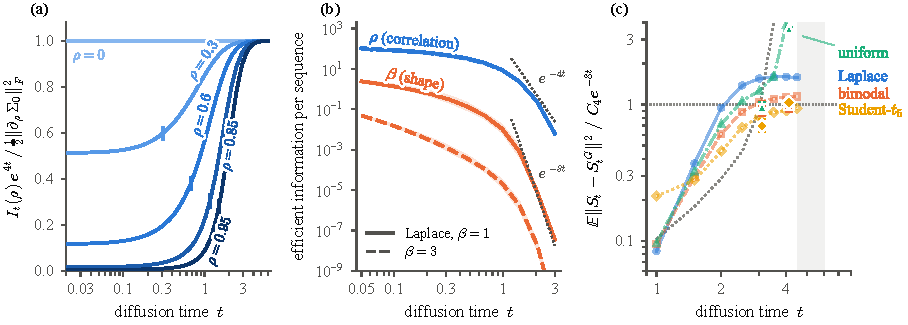
\includegraphics[width=\textwidth]{fig_theory.pdf}
  \caption{The paper's theory figure (Section 3), reproduced for reference. (a)
  Exact Fisher information of the Gaussian chain about $\corr$ divided by its
  asymptote $\tfrac12\Frob{\partial_\corr\Sig_0}^2e^{-4t}$, five correlations, ticks at
  $\tstar(\corr)$ (\cref{prop:att:gaussinfo,prop:att:tstar}). (b) Efficient
  information per sequence about $\corr$ (degree two) and about the shape exponent
  $\beta$ (degree four) of the generalised-Gaussian chain, from Fisher-identity scores,
  against the guides $e^{-4t}$ and $e^{-8t}$ (\cref{sec:att:information}). (c) The
  closure gap $\E\lVert\score-\Sgauss\rVert^2$ divided by $\tfrac16\Frob{\kfour}^2e^{-8t}$
  for four innovation families (\cref{prop:att:c4}), with the large-sample constants
  and the double-precision floor.}
  \label{fig:att:theory}
\end{figure}

\Cref{fig:att:theory} is the paper's Figure in Section 3. Panel (a) is
\cref{prop:att:gaussinfo}: no Monte Carlo, a closed form on a fine grid of $t$
(\code{part\_gauss} of \code{experiments/e01\_information\_decay.py}); the curves
reach one, and the tick marks show that a strongly correlated chain approaches its
asymptote later, as $\alpha^2\lmax$ requires. Panel (b) is
\cref{prop:att:info2,prop:att:info4} measured on the chain: the per-sequence scores of
the marginal likelihood are obtained by Fisher's identity through the tree-exact
recursion (\code{per\_chain\_scores} in \code{src/markov\_score/information.py}), the
outer-product matrix is inverted for the efficient information, and the slopes above
$\tstar$ are compared with $-4$ and $-8$; the constant of the shape rate is verified
to high precision only in the scalar case (E21), because the outer-product estimate on
the chain is a small residual of order-one quantities and reaches a quadrature floor.
Panel (c) is \cref{prop:att:c4}: the gap is measured by tree-exact message passing
against the LMMSE twin, divided by the predicted constant, on a domain wide enough
for each family's sample (E18), with the bootstrap intervals from many sequences
because the per-sequence gap is heavy-tailed (a degree-six polynomial in nearly
Gaussian variables). The uniform family, with the smallest constant, reaches the
double-precision floor of the posterior means first. All numbers are in the paper;
none is repeated here.

\section{Worked examples}
\label{sec:att:examples}

\begin{example}[The scalar Laplace law]
\label{ex:att:laplace}
A unit-variance Laplace variable has excess kurtosis $3$, so $\kappa_4=3$ and the
constant of \cref{eq:att:scoregap} is $\kappa_4^2/6=1.5$. The leading term of the score
gap is $\tfrac{3}{6}\Hen3(x)e^{-4t}=\tfrac12(x^3-3x)e^{-4t}$; at $x=2$ and $t=1$ it is
$\tfrac12\cdot2\cdot e^{-4}=0.0183$, against a twin score of $-2$. The expected squared
gap at $t=2$ is $1.5\,e^{-16}=1.5\times1.13\times10^{-7}=1.7\times10^{-7}$, and since
the score energy at that level is close to one (\cref{prop:ou:energy}), the relative
score error of the twin is about $\sqrt{1.7\times10^{-7}}=4\times10^{-4}$.
\end{example}

\begin{example}[The shape constant at the Gaussian member]
\label{ex:att:shape}
The generalised Gaussian $\innov_\beta\propto e^{-|\varepsilon/s_\beta|^\beta}$ at unit
variance has excess kurtosis $\kappa(\beta)=\Gamma(5/\beta)\Gamma(1/\beta)/\Gamma(3/\beta)^2-3$.
Its derivative at the Gaussian member $\beta=2$ can be done by hand with the digamma
recursion $\psi(x+1)=\psi(x)+1/x$:
$\frac{\dd}{\dd\beta}\log(\kappa+3)=\beta^{-2}[-5\psi(5/\beta)-\psi(1/\beta)+6\psi(3/\beta)]$,
and at $\beta=2$, with $\psi(5/2)=\psi(1/2)+2+\tfrac23$ and $\psi(3/2)=\psi(1/2)+2$,
the bracket is $(-5-1+6)\psi(\tfrac12)-\tfrac{40}3+12=-\tfrac43$, so the derivative
of the logarithm is $-\tfrac13$ and $\partial_\beta\kappa|_{\beta=2}=3\times(-\tfrac13)=-1$
exactly. In the scalar case \cref{eq:att:info4} therefore predicts
$I_t(\beta)=\tfrac1{24}e^{-8t}(1+O(e^{-2t}))$ at the Gaussian member: an information of
one part in twenty-four times $e^{-8t}$ per observation. The paper's E21 checks this
constant by untruncated quadrature (Appendix E).
\end{example}

\begin{example}[The two-site Gaussian chain, exactly]
\label{ex:att:twosite}
For $\nsites=2$, $\Sig_0=\begin{psmallmatrix}1&\corr\\\corr&1\end{psmallmatrix}$ and
$\partial_\corr\Sig_0=\begin{psmallmatrix}0&1\\1&0\end{psmallmatrix}$, so
$\tfrac12\Frob{\partial_\corr\Sig_0}^2=1$. With $\Sig_t=\begin{psmallmatrix}1&\alpha^2\corr\\\alpha^2\corr&1\end{psmallmatrix}$,
$\Sig_t^{-1}\partial_\corr\Sig_t=\frac{\alpha^2}{1-\alpha^4\corr^2}\begin{psmallmatrix}-\alpha^2\corr&1\\1&-\alpha^2\corr\end{psmallmatrix}$,
whose square has trace $2\alpha^4(1+\alpha^4\corr^2)/(1-\alpha^4\corr^2)^2$, so by
\cref{prop:att:gaussinfo}
\[
  I_t(\corr)=\frac{\alpha^4(1+\alpha^4\corr^2)}{(1-\alpha^4\corr^2)^2}=e^{-4t}\bigl(1+3\alpha^4\corr^2+O(\alpha^8)\bigr).
\]
At $\corr=0.85$ and $t=1$: $\alpha^4=e^{-4}=0.01832$ and $\alpha^4\corr^2=0.01323$, so
\[
  I_1=\frac{0.01832\times1.01323}{0.98677^2}=0.01906,
\]
four per cent above the asymptote. Here
the correction is $O(\alpha^4)$ rather than $O(\alpha^2)$ because $\tr(\Sig_0-\Id)=0$
and the first-order term of the Neumann series drops out of the trace; for the
$32$-site chain it does not, and the correction is $O(\alpha^2\lmax)$.
\end{example}

\begin{example}[The fourth-cumulant tensor of a three-site chain]
\label{ex:att:tensor}
Let $a_1\sim\normal01$, $a_2=\corr a_1+\varepsilon_2$, $a_3=\corr a_2+\varepsilon_3=\corr^2a_1+\corr\varepsilon_2+\varepsilon_3$,
with i.i.d.\ innovations of variance $\ivar=1-\corr^2$ and fourth cumulant
$\kappa_4(\varepsilon)=3\ivar^2$ (Laplace). Joint cumulants are additive over the
independent summands and $a_1$ is Gaussian, so
$\kfour[ijkl]=\kappa_4(\varepsilon)\sum_{m=2}^{\min(i,j,k,l)}\corr^{i+j+k+l-4m}$
(\code{chain\_kappa4} in \code{src/markov\_score/theory.py}). The nonzero entries up
to permutation are $\kfour[2222]=3\ivar^2$, $\kfour[2223]=3\ivar^2\corr$,
$\kfour[2233]=3\ivar^2\corr^2$, $\kfour[2333]=3\ivar^2\corr^3$ and
$\kfour[3333]=3\ivar^2(\corr^4+1)$. Over ordered tuples the Frobenius norm is
\[
  \Frob{\kfour}^2=9\ivar^4\bigl[1+4\corr^2+6\corr^4+4\corr^6+(1+\corr^4)^2\bigr],
\]
the multiplicities being $1,4,6,4,1$. At $\corr=0.85$: $\ivar=0.2775$, $\ivar^4=0.00593$,
$\corr^2=0.7225$, $\corr^4=0.5220$, $\corr^6=0.3772$; the bracket is
$1+2.890+3.132+1.509+2.317=10.85$, so $\Frob{\kfour}^2=9\times0.00593\times10.85=0.579$
and $\tfrac16\Frob{\kfour}^2=0.0965$. The same recipe at $\nsites=32$ gives the
constant the paper quotes for the Laplace chain (Section 3, ``Verification with the
exact score''), which grows linearly in $\nsites$ away from the first site.
\end{example}

\begingroup\setlength{\emergencystretch}{2em}
\where{Section 3 of the paper (Theorems 2--4, Assumption (E), Corollary 5, the
crossover and heavy-tail paragraphs, the Edgeworth paragraph) and Appendix A
(the proofs). Experiments: E01 (Gaussian closed form, shape information on the chain,
closure gap), E16 (Edgeworth correction), E18 (closure constant and heavy tails on
wide domains, untruncated scalar quadrature), E21 (information curve at $\corr=0.5$
and the scalar shape constant). Code: \code{src/\allowbreak markov\_score/\allowbreak theory.py}
(\code{he}, \code{chain\_\allowbreak covariance}, \code{chain\_\allowbreak kappa4}, \code{gaussian\_\allowbreak chain\_\allowbreak fisher},
\code{score\_\allowbreak gap\_\allowbreak constant}, \code{shape\_\allowbreak information\_\allowbreak constant},
\code{correlation\_\allowbreak information\_\allowbreak constant}, \code{crossover\_\allowbreak time}),
\code{src/\allowbreak markov\_score/\allowbreak information.py} (\code{per\_\allowbreak chain\_\allowbreak scores},
\code{outer\_\allowbreak product\_\allowbreak information}, \code{efficient\_\allowbreak information}),
\code{experiments/\allowbreak e01\_information\_decay.py},
\code{experiments/\allowbreak e16\_edgeworth\_oracle.py},
\code{experiments/\allowbreak e18\_closure\_wide.py},
\code{experiments/\allowbreak e21\_information\_curve.py}; the Lean targets for the
constants are listed in \code{lean/\allowbreak README.md}. Audit: \code{docs/\allowbreak SCIENCE\_\allowbreak AUDIT.md},
\code{reports/\allowbreak audit-\allowbreak 2026-\allowbreak 09-\allowbreak 18.tex}, Section 3.}
\endgroup

\paragraph{References.}
F.~G.~Mehler, 1866, ``Ueber die Entwicklung einer Function von beliebig vielen
Variabeln nach Laplaceschen Functionen h\"oherer Ordnung'', Journal f\"ur die reine und
angewandte Mathematik 66, 161--176.
S.~Janson, 1997, \emph{Gaussian Hilbert Spaces}, Cambridge University Press (Wick
products and Wick's theorem, Chapter 3).
P.~McCullagh, 1987, \emph{Tensor Methods in Statistics}, Chapman and Hall (joint
cumulants, the Leonov--Shiryaev formula, Edgeworth expansions).
A.~W.~van der Vaart, 1998, \emph{Asymptotic Statistics}, Cambridge University Press
(local asymptotic minimax theorem, Chapter 8).
D.~Guo, S.~Shamai and S.~Verd\'u, 2005, ``Mutual information and minimum mean-square
error in Gaussian channels'', IEEE Transactions on Information Theory 51, 1261--1282.
A.~Katsevich and A.~S.~Bandeira, 2023, ``Likelihood maximization and moment matching
in low SNR Gaussian mixture models'', Communications on Pure and Applied Mathematics
76, 788--842.
